
\section{Appendix}

\subsection{Figures}

\begin{figure}[H]
	\centering
	\subfloat[\centering Predicted]{{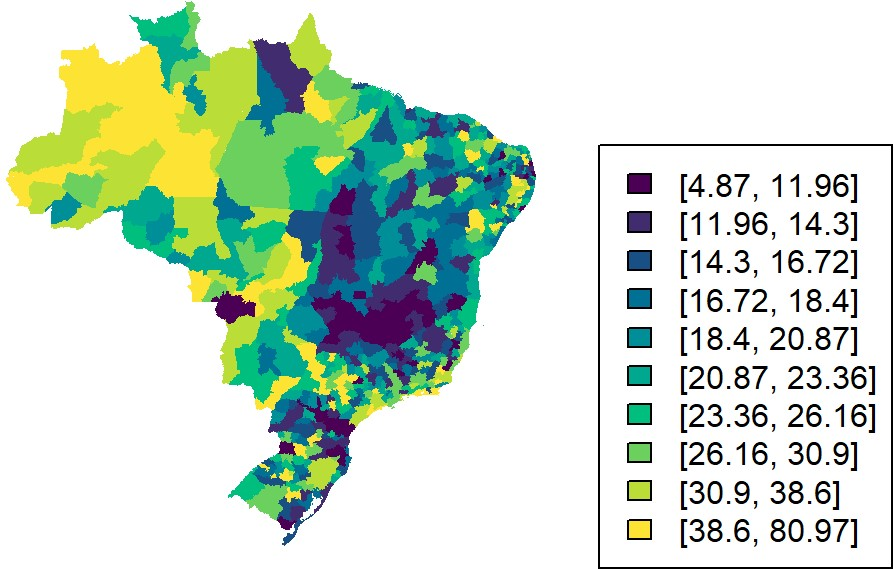
\includegraphics[scale=0.6]{pred_TB_rate_map.jpg} }}%
	\qquad
	\subfloat[\centering True]{{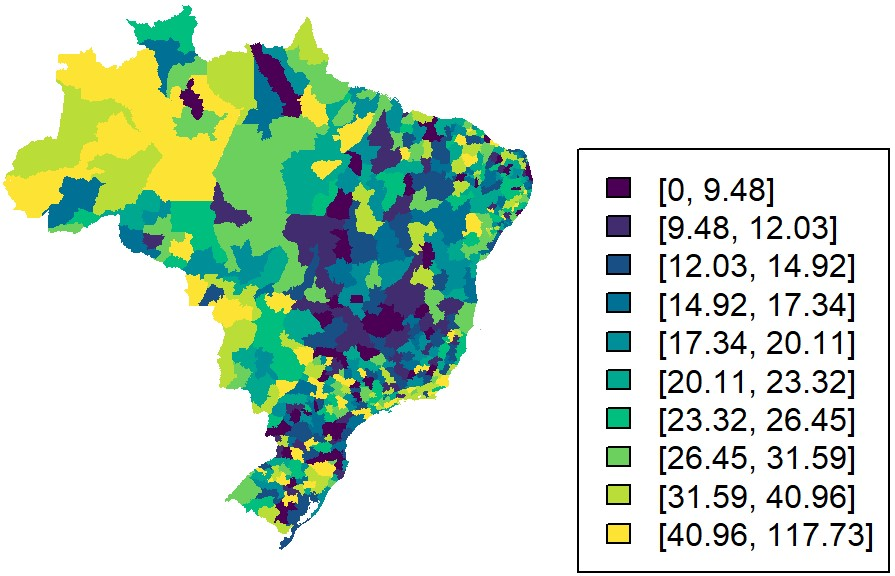
\includegraphics[scale=0.6]{true_TB_rate_map.jpg} }}%
	\caption{Predicted (a) and True (b) rates of TB per 100k inhabitants. North-western parts of the country as well as parts near the south exhibit high TB incidence per capita. These would roughly correspond to the states (\textit{estados}) of Amazonas in the North-West, Sao Paolo in the South and Rio de Janeiro on the South East coast. Refer to state map in Figure \ref{fig:brazil-division-states}}%
	\label{fig:pred_TB_rate_map}%
\end{figure}

\begin{figure}[H]
\centering
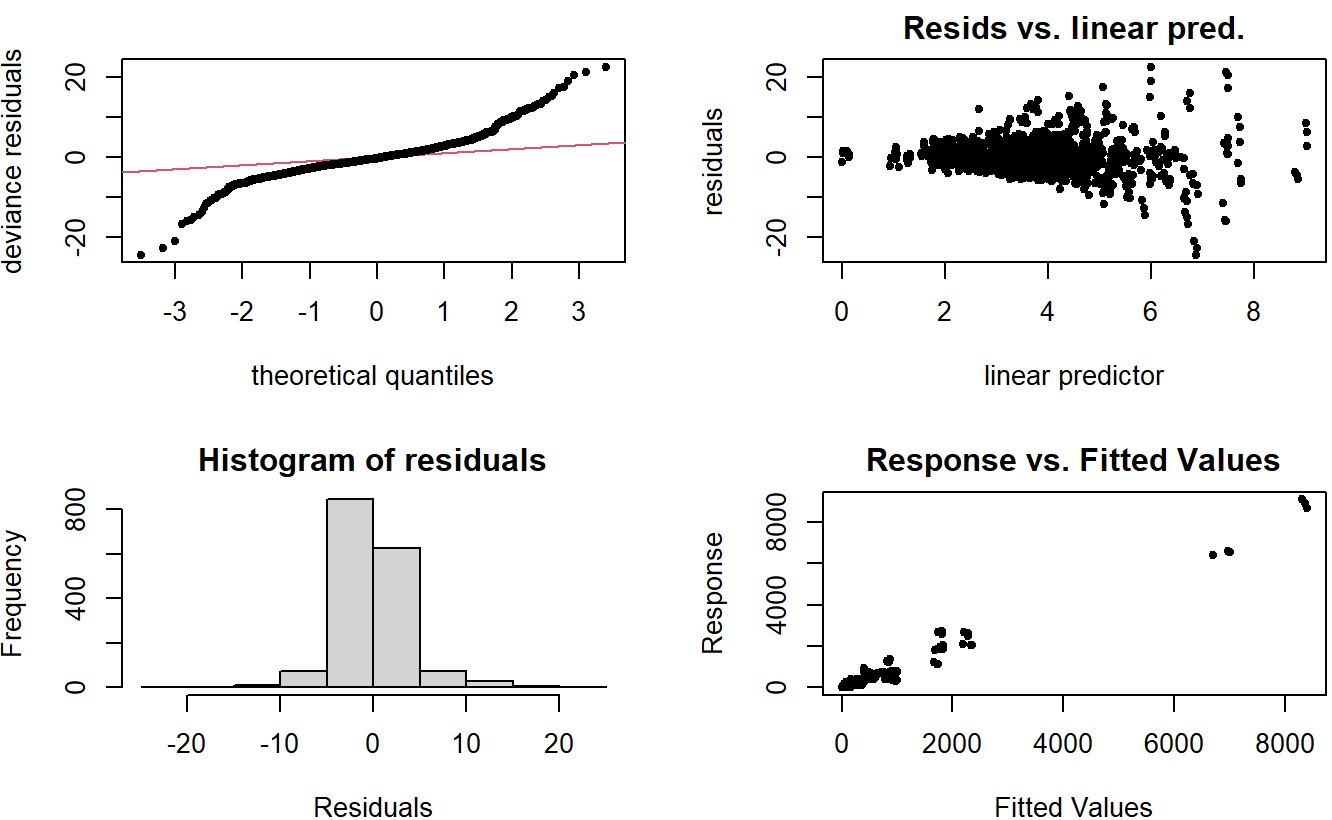
\includegraphics[scale=0.5]{model_poisson_check.jpg}
\caption{\label{fig:model_poisson_check}\texttt{gam.check( )} results for \texttt{model\_poisson}. The data is overdispersed as can be seen from both the QQ-plot and the fanning of the Resids vs linear pred. plot. The histogram of residuals is also quite different from a gaussian distribution}
\end{figure}

\begin{figure}[H]
\centering
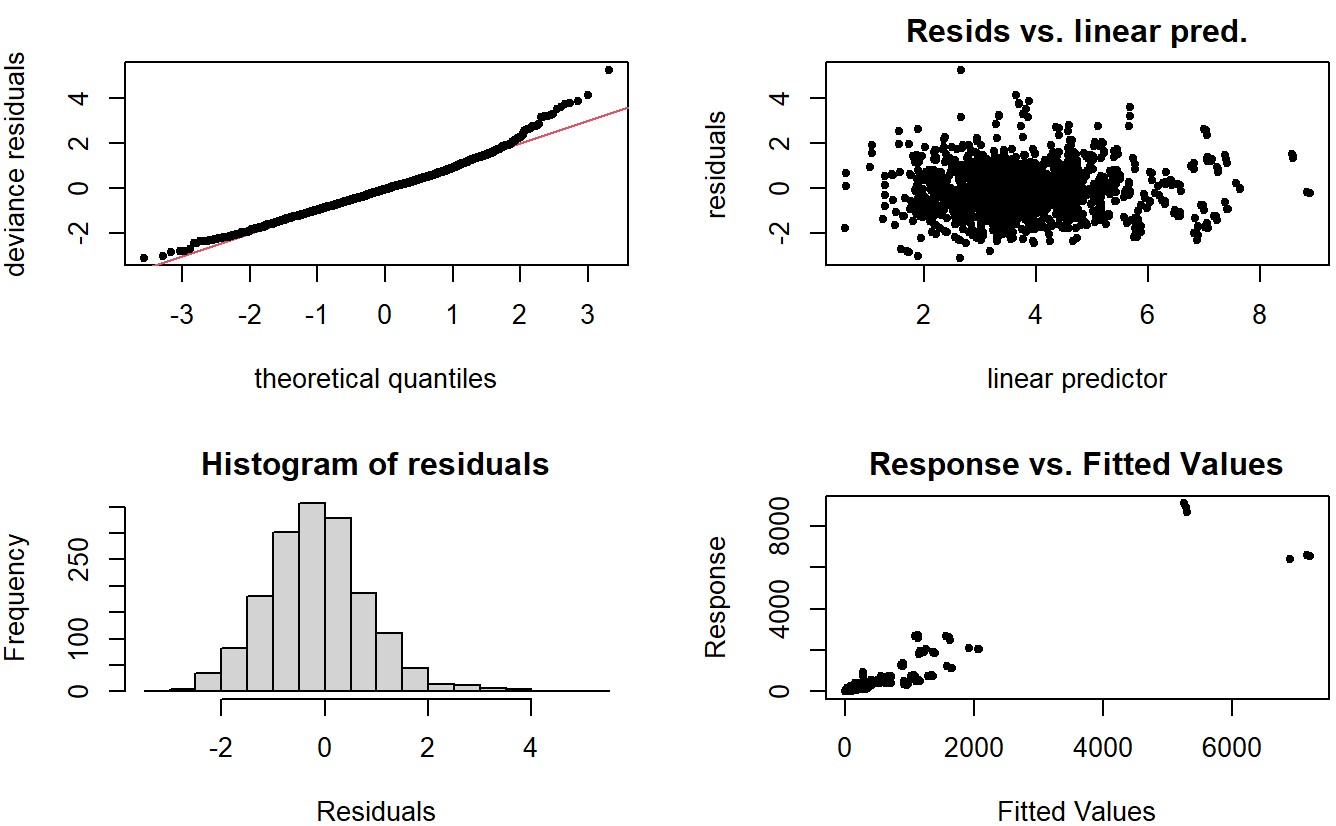
\includegraphics[scale=0.5]{model_nb_2_check.jpg}
\caption{\label{fig:model_nb_2_check}\texttt{gam.check( )} results for \texttt{model\_nb\_2}. Albeit an improvement of the Poisson model, the model has a tough time correctly predicting values on the upper and lower quantiles}
\end{figure}

\begin{figure}[H]
\centering
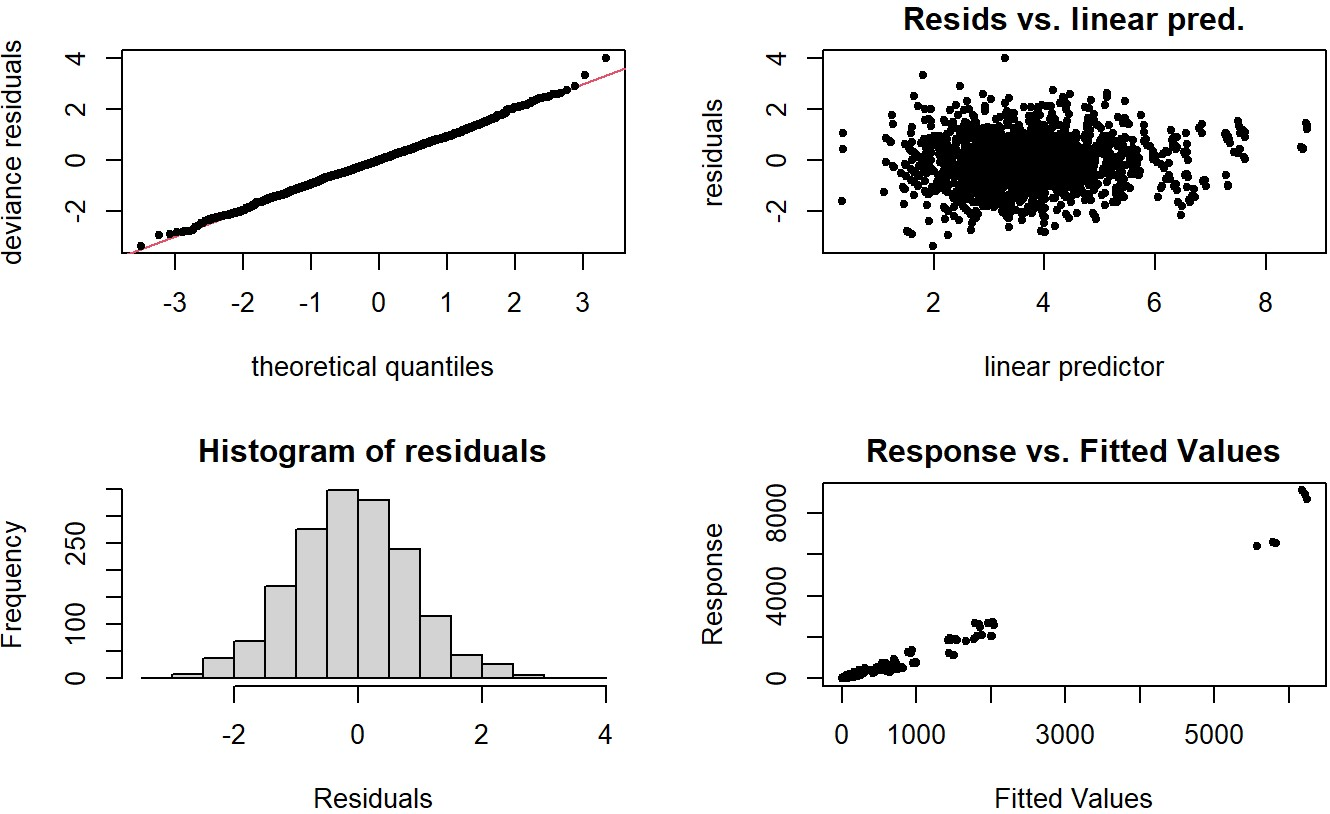
\includegraphics[scale=0.5]{spatial_model_2_check.jpg}
\caption{\label{fig:spatial_model_2_check}\texttt{gam.check( )} results for \texttt{spatial.model.2}. This is the model that has finally been used as temporal additions on top of this provide very little additional explanatory power}
\end{figure}


%\begin{figure}[H]
%\centering
%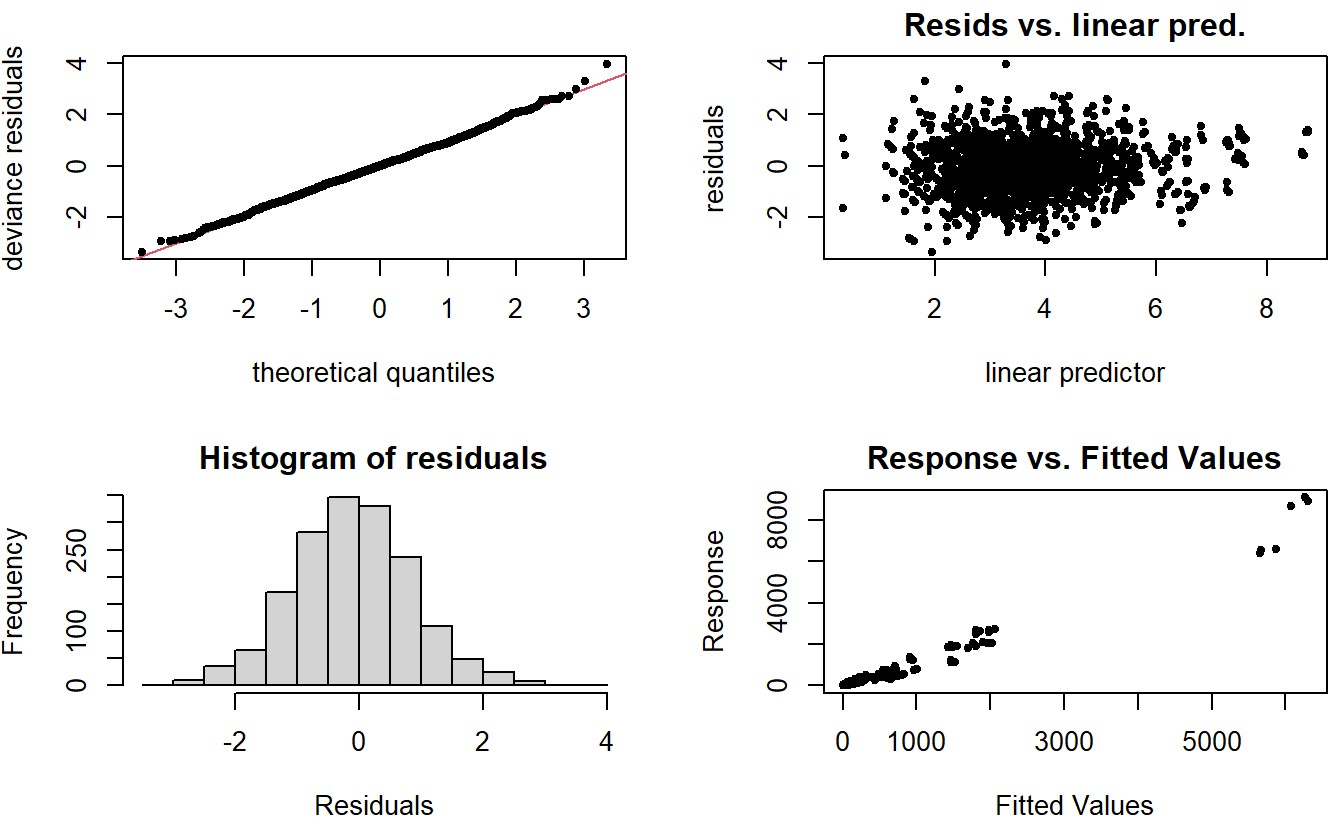
\includegraphics[scale=0.5]{spatio_temporal_model_2_check.jpg}
%\caption{\label{fig:spatio_temporal_model_2_check}\texttt{gam.check( )} results for \texttt{spatial.temporal.model.2}}
%\end{figure}

\begin{figure}[H]
\centering
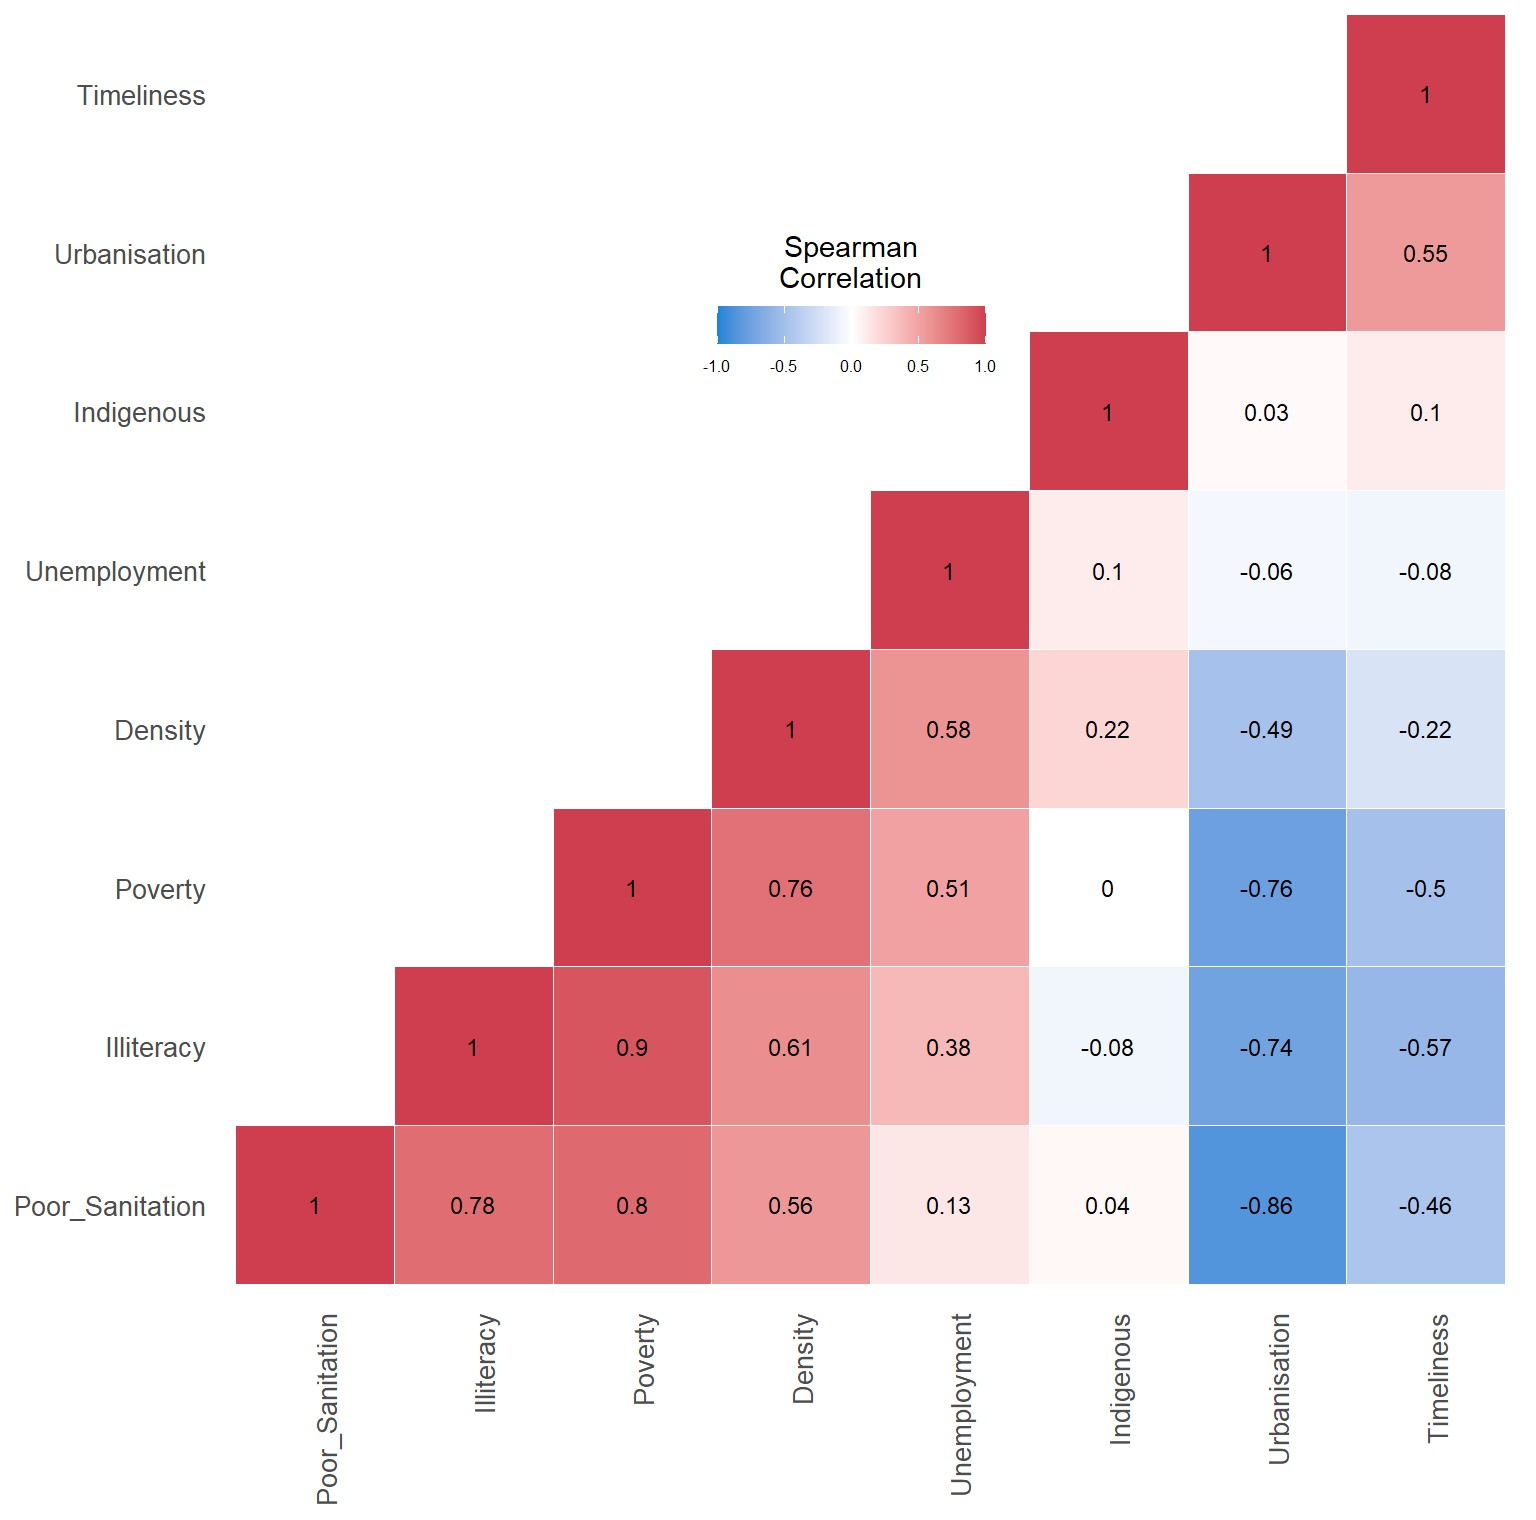
\includegraphics[scale=0.4]{spearman_correl.jpg}
\caption{\label{fig:spearman_correl}Correlogram shows covariates with highest positive and negative correlations.}
\end{figure}

\begin{figure}[H]
\centering
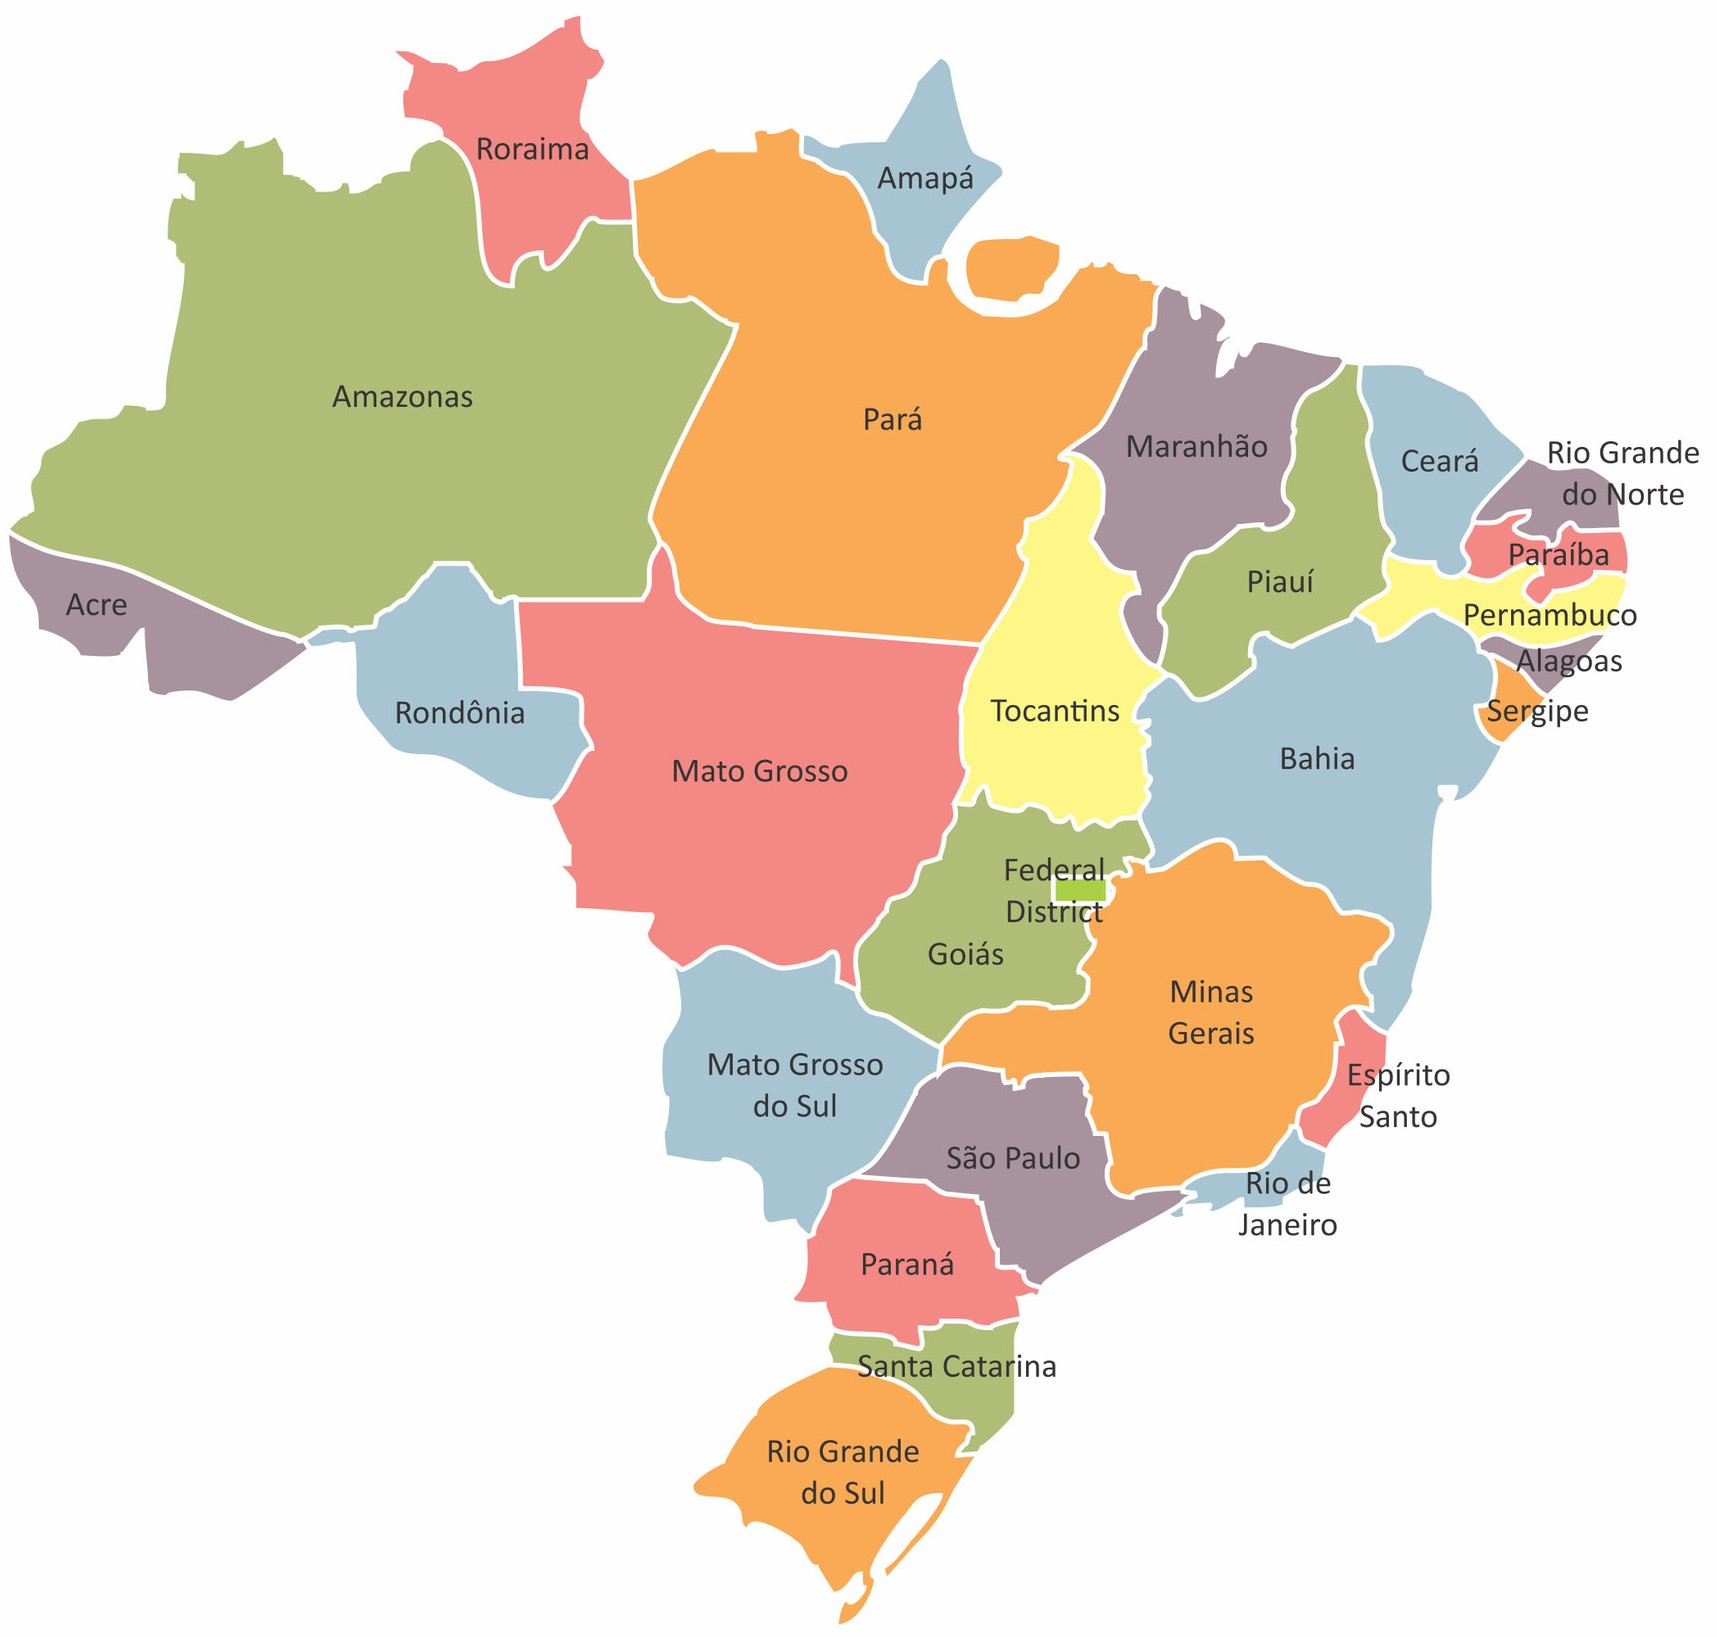
\includegraphics[scale=0.5]{brazil-division-states.jpg}
\caption{\label{fig:brazil-division-states}State map of Brazil provided for reference.}
\end{figure}


\subsection{Tables}

\begin{table}[H]
\centering
\begin{tabular}{l|c|c}
Model & AIC & Deviance Explained\\\hline
\texttt{model\_poisson} & 34047.36 & 66.9\%\\
\texttt{model\_nb} & 14391.19 & 43.9\%\\
\texttt{model\_nb\_2} & 14389.56 & 43.9\%\\
\texttt{model\_nb\_3} & 14405.00 & 43.0\%\\
\texttt{model\_nb\_time} & 14389.70 & 44.0\%\\
\texttt{temporal.model} & 14390.43 & 44.0\%\\
\texttt{spatial.model} & 14013.13 & 56.4\%\\
\textcolor{teal}{\texttt{spatial.model.2}} & \textcolor{teal}{13650.8} & \textcolor{teal}{69.9\%}\\
\texttt{spatial.model.temporal} & 14227.12 & 52.2\%\\
\texttt{spatial.model.temporal.2} & 13647.93 & 70.1\%
\end{tabular}
\caption{\label{tab:metrics}Comparison of models.}
\end{table}

\subsection{Code}
\begin{minted}[
frame=lines,
framesep=2mm,
baselinestretch=1.2,
bgcolor=LightGray,
fontsize=\footnotesize,
linenos
]{R}
# Load Data
load("datasets_project.RData")
# Import Libraries
library(mgcv) # required for GAM 

#fit poisson model with socio-economic variables
model_poisson <- gam(formula = TB ~ offset(log(Population)) + s(Indigenous)
+ s(Illiteracy) + s(Urbanisation) + s(Density) + s(Poverty) + s(Poor_Sanitation)
+ s(Unemployment) + s(Timeliness), 
data = TBdata, 
family = poisson(link = 'log')
)

#add flexibility
model_poisson.more.knots <- gam(formula = TB ~ offset(log(Population)) + s(Indigenous, k = 60) 
+ s(Illiteracy, k = 60) +  s(Urbanisation, k = 60) + s(Density, k = 60) 
+ s(Poverty, k = 60) + s(Poor_Sanitation, k = 60) + s(Unemployment, k = 60) 
+ s(Timeliness, k = 60), 
data = TBdata, 
family = poisson(link = 'log')
)

#fit negative binomial model with  socioeconomic
model_nb <- gam(formula = TB ~ offset(log(Population)) + s(Indigenous) 
+  s(Illiteracy) + s(Urbanisation) + s(Density) + s(Poverty) + s(Poor_Sanitation)
+ s(Unemployment) + s(Timeliness), 
data = TBdata, family = nb(link = 'log')
)

#fit a linear relation between squared residuals and prediction to see whether another model describes
#the variance-fitted values relation better
summary(lm(log(model_nb$residuals^2) ~ log(predict(model_nb, type = 'response'))))

#drop Illiteracy
model_nb_2 <- gam(formula = TB ~ offset(log(Population)) + s(Indigenous) +  s(Urbanisation) + s(Density) 
+ s(Poverty) + s(Poor_Sanitation) + s(Unemployment) + s(Timeliness),
data = TBdata,
family = nb(link = 'log')
)

# Likelihood ratio test
anova.gam(model_nb_2, model_nb, test = 'F') # p-value is over 0.05
# The models are statistically indistinguishable

model_nb_3 <- gam(formula = TB ~ offset(log(Population)) + s(Indigenous) +  s(Urbanisation) + s(Density) 
+ s(Poor_Sanitation) + s(Unemployment) + s(Timeliness), 
data = TBdata, 
family = nb(link = 'log')
)
# Likelihood ratio test
anova.gam(model_nb_3, model_nb_2, test = 'F')# p-value is less than 0.05
# The models are statistically different. Poverty should not be excluded.

### Model chosen (with socio-economic covariates) is the negative binomial without Illiteracy
### as the effect of illiteracy cannot be reliably stated to be non-zero

#### Introducing temporality as a grouping variable
#Temporal model
model_nb_time <- gam(formula = TB ~ offset(log(Population)) + s(Indigenous, by = Year) 
+ s(Urbanisation, by = Year) + s(Density, by = Year) + s(Poverty, by = Year) + s(Poor_Sanitation, by = Year) 
+ s(Unemployment, by = Year) + s(Timeliness, by = Year), 
data = TBdata, 
family = nb(link = 'log')
)

#### Temporality as a covariate
TBdata$Year.asFactor <- factor(TBdata$Year)

temporal.model <- gam(formula = TB ~ offset(log(Population)) + s(Indigenous)
+ s(Urbanisation) + s(Density) + s(Poor_Sanitation) + s(Unemployment) + s(Poverty)
+ s(Timeliness) + Year.asFactor,
data = TBdata ,
family = nb(link = 'log')
)

### Adding spatial covariates
spatial.model <- gam(formula = TB ~ offset(log(Population)) + s(Indigenous) 
+ s(Urbanisation) + s(Density) + s(Poor_Sanitation) + s(Unemployment) +s(Poverty)
+ s(Timeliness) + s(lon , lat),
data = TBdata , 
family = nb(link = 'log')
)

### Using separate smoothers
spatial.model.2 <- gam(formula = TB ~ offset(log(Population)) + s(Indigenous) 
+ s(Urbanisation) + s(Density) + s(Poor_Sanitation) + s(Unemployment) + s(Poverty)
+ s(Timeliness) + te(lon , lat , k = 20),
data = TBdata , 
family = nb(link = 'log')
)

# Check if this model is significantly different from one with only socio-economic covariates
anova.gam(spatial.model.2, model_nb_2, test = 'LRT')

#### Spatio-temporal model
spatio.temporal.model <- gam(formula = TB ~ offset(log(Population)) + s(Urbanisation, by = Year.asFactor) 
+ s(Density, by = Year.asFactor) + s(Poverty, by = Year.asFactor) 
+ s(Poor_Sanitation, by = Year.asFactor) + s(Timeliness, by = Year.asFactor) 
+ s(Unemployment, by = Year.asFactor) + te(lon,lat, by = Year.asFactor), data = TBdata, family = nb(link = 'log'))

### Spatio-temporal model (with Year as parametric covariate)
spatio.temporal.model.2 <- gam(formula = TB ~ offset(log(Population)) + s(Indigenous) 
+ s(Urbanisation) + s(Density) + s(Poor_Sanitation) + s(Unemployment) + s(Poverty)
+ s(Timeliness) + te(lon , lat , k = 20) + Year.asFactor,
data = TBdata , 
family = nb(link = 'log')
)
\end{minted}


\subsection{Model Summaries and Residual Checks}
\begin{minted}[
frame=lines,
framesep=2mm,
baselinestretch=1.2,
bgcolor=LightGray,
fontsize=\footnotesize,
linenos
]{R}
# check summary
summary(model_poisson)

Family: poisson 
Link function: log 

Formula:
TB ~ offset(log(Population)) + s(Indigenous) + s(Illiteracy) + 
    s(Urbanisation) + s(Density) + s(Poverty) + s(Poor_Sanitation) + 
    s(Unemployment) + s(Timeliness)

Parametric coefficients:
             Estimate Std. Error z value Pr(>|z|)    
(Intercept) -8.449827   0.004199   -2012   <2e-16 ***
---
Signif. codes:  0 ‘***’ 0.001 ‘**’ 0.01 ‘*’ 0.05 ‘.’ 0.1 ‘ ’ 1

Approximate significance of smooth terms:
                     edf Ref.df Chi.sq p-value    
s(Indigenous)      8.961  8.999  569.4  <2e-16 ***
s(Illiteracy)      8.989  9.000 2704.0  <2e-16 ***
s(Urbanisation)    8.900  8.996 1490.4  <2e-16 ***
s(Density)         8.985  9.000 1758.4  <2e-16 ***
s(Poverty)         8.956  8.999 1470.2  <2e-16 ***
s(Poor_Sanitation) 8.979  9.000 1327.0  <2e-16 ***
s(Unemployment)    8.993  9.000 2423.5  <2e-16 ***
s(Timeliness)      8.352  8.864  600.7  <2e-16 ***
---
Signif. codes:  0 ‘***’ 0.001 ‘**’ 0.01 ‘*’ 0.05 ‘.’ 0.1 ‘ ’ 1

R-sq.(adj) =  0.976   Deviance explained = 0.669
UBRE = 13.899  Scale est. = 1         n = 1671

model_poisson$aic
34047.36

# Excerpt from residual check
gam.check(model_poisson)

                     k`  edf k-index p-value    
s(Indigenous)      9.00 8.96    0.39  <2e-16 ***
s(Illiteracy)      9.00 8.99    0.41  <2e-16 ***
s(Urbanisation)    9.00 8.90    0.41  <2e-16 ***
s(Density)         9.00 8.98    0.39  <2e-16 ***
s(Poverty)         9.00 8.96    0.39  <2e-16 ***
s(Poor_Sanitation) 9.00 8.98    0.40  <2e-16 ***
s(Unemployment)    9.00 8.99    0.39  <2e-16 ***
s(Timeliness)      9.00 8.35    0.43  <2e-16 ***
---

#check summary
summary(model_nb_2)

Family: Negative Binomial(6.146) 
Link function: log 

Formula:
TB ~ offset(log(Population)) + s(Indigenous) + s(Urbanisation) + 
    s(Density) + s(Poverty) + s(Poor_Sanitation) + s(Unemployment) + 
    s(Timeliness)

Parametric coefficients:
            Estimate Std. Error z value Pr(>|z|)    
(Intercept) -8.42863    0.01094  -770.6   <2e-16 ***
---
Signif. codes:  0 ‘***’ 0.001 ‘**’ 0.01 ‘*’ 0.05 ‘.’ 0.1 ‘ ’ 1

Approximate significance of smooth terms:
                     edf Ref.df Chi.sq  p-value    
s(Indigenous)      1.518  1.833  21.13 2.08e-05 ***
s(Urbanisation)    6.610  7.752  23.73  0.00167 ** 
s(Density)         4.578  5.667 147.64  < 2e-16 ***
s(Poverty)         5.771  6.945  21.36  0.00394 ** 
s(Poor_Sanitation) 6.119  7.293  76.07  < 2e-16 ***
s(Unemployment)    5.776  6.977  64.21  < 2e-16 ***
s(Timeliness)      4.106  5.103  66.42  < 2e-16 ***
---
Signif. codes:  0 ‘***’ 0.001 ‘**’ 0.01 ‘*’ 0.05 ‘.’ 0.1 ‘ ’ 1

R-sq.(adj) =   0.86   Deviance explained = 0.439
-REML = 7234.9  Scale est. = 1         n = 1671

model_nb_2$aic
14389.56

# Excerpt from residual check
gam.check(model_nb_2)

                     k`  edf k-index p-value    
s(Indigenous)      9.00 1.52    0.49  <2e-16 ***
s(Urbanisation)    9.00 6.61    0.50  <2e-16 ***
s(Density)         9.00 4.58    0.50  <2e-16 ***
s(Poverty)         9.00 5.77    0.49  <2e-16 ***
s(Poor_Sanitation) 9.00 6.12    0.50  <2e-16 ***
s(Unemployment)    9.00 5.78    0.50  <2e-16 ***
s(Timeliness)      9.00 4.11    0.56  <2e-16 ***
---

# check summary
summary(spatial.model.2)

Family: Negative Binomial(12.246) 
Link function: log 

Formula:
TB ~ offset(log(Population)) + s(Indigenous) + s(Urbanisation) + 
    s(Density) + s(Poor_Sanitation) + s(Unemployment) + s(Poverty) + 
    s(Timeliness) + te(lon, lat, k = 20)

Parametric coefficients:
             Estimate Std. Error z value Pr(>|z|)    
(Intercept) -8.467186   0.008485  -997.9   <2e-16 ***
---
Signif. codes:  0 ‘***’ 0.001 ‘**’ 0.01 ‘*’ 0.05 ‘.’ 0.1 ‘ ’ 1

Approximate significance of smooth terms:
                       edf  Ref.df  Chi.sq  p-value    
s(Indigenous)        3.700   4.346   19.53 0.000922 ***
s(Urbanisation)      5.188   6.221   52.90  < 2e-16 ***
s(Density)           4.107   5.012   38.40 1.58e-06 ***
s(Poor_Sanitation)   5.367   6.412   27.55 0.000174 ***
s(Unemployment)      4.132   5.125   79.61  < 2e-16 ***
s(Poverty)           6.716   7.729   42.69  < 2e-16 ***
s(Timeliness)        2.445   3.053   46.59  < 2e-16 ***
te(lon,lat)        139.341 174.137 1088.66  < 2e-16 ***
---
Signif. codes:  0 ‘***’ 0.001 ‘**’ 0.01 ‘*’ 0.05 ‘.’ 0.1 ‘ ’ 1

R-sq.(adj) =  0.926   Deviance explained = 0.699
-REML = 6987.8  Scale est. = 1         n = 1671

spatial.model.2$aic
13650.8

#Excerpt from residual check
gam.check(spatial.model.2)

                       k`    edf k-index p-value    
s(Indigenous)        9.00   3.70    0.63  <2e-16 ***
s(Urbanisation)      9.00   5.19    0.61  <2e-16 ***
s(Density)           9.00   4.11    0.63  <2e-16 ***
s(Poor_Sanitation)   9.00   5.37    0.61  <2e-16 ***
s(Unemployment)      9.00   4.13    0.62  <2e-16 ***
s(Poverty)           9.00   6.72    0.61  <2e-16 ***
s(Timeliness)        9.00   2.45    0.66  <2e-16 ***
te(lon,lat)        399.00 139.34    0.65  <2e-16 ***
---

# check summary
summary(spatio.temporal.model.2)

Family: Negative Binomial(12.299) 
Link function: log 

Formula:
TB ~ offset(log(Population)) + s(Indigenous) + s(Urbanisation) + 
    s(Density) + s(Poor_Sanitation) + s(Unemployment) + s(Poverty) + 
    s(Timeliness) + te(lon, lat, k = 20) + Year.asFactor

Parametric coefficients:
                    Estimate Std. Error  z value Pr(>|z|)    
(Intercept)       -8.4532889  0.0144206 -586.197   <2e-16 ***
Year.asFactor2013 -0.0005816  0.0201595   -0.029    0.977    
Year.asFactor2014 -0.0417054  0.0202005   -2.065    0.039 *  
---
Signif. codes:  0 ‘***’ 0.001 ‘**’ 0.01 ‘*’ 0.05 ‘.’ 0.1 ‘ ’ 1

Approximate significance of smooth terms:
                       edf  Ref.df  Chi.sq  p-value    
s(Indigenous)        3.702   4.347   19.56 0.000912 ***
s(Urbanisation)      5.197   6.230   53.05  < 2e-16 ***
s(Density)           4.107   5.011   38.45 1.89e-06 ***
s(Poor_Sanitation)   5.374   6.418   27.61 0.000170 ***
s(Unemployment)      4.145   5.140   80.03  < 2e-16 ***
s(Poverty)           6.722   7.734   42.72  < 2e-16 ***
s(Timeliness)        2.460   3.070   46.59  < 2e-16 ***
te(lon,lat)        139.707 174.516 1093.31  < 2e-16 ***
---
Signif. codes:  0 ‘***’ 0.001 ‘**’ 0.01 ‘*’ 0.05 ‘.’ 0.1 ‘ ’ 1

R-sq.(adj) =  0.926   Deviance explained = 0.701
-REML = 6991.1  Scale est. = 1         n = 1671

spatio.temporal.model.2$aic
13647.93

#Excerpt from residual check
gam.check(spatio.temporal.model.2)

                       k`    edf k-index p-value    
s(Indigenous)        9.00   3.70    0.63  <2e-16 ***
s(Urbanisation)      9.00   5.20    0.60  <2e-16 ***
s(Density)           9.00   4.11    0.62  <2e-16 ***
s(Poor_Sanitation)   9.00   5.37    0.61  <2e-16 ***
s(Unemployment)      9.00   4.15    0.61  <2e-16 ***
s(Poverty)           9.00   6.72    0.61  <2e-16 ***
s(Timeliness)        9.00   2.46    0.66  <2e-16 ***
te(lon,lat)        399.00 139.71    0.64  <2e-16 ***
---
\end{minted}